\documentclass[lettersize,journal]{IEEEtran}
\usepackage{amsmath,amsfonts}
\usepackage{algorithmic}
\usepackage{algorithm}
\usepackage{array}
\usepackage[caption=false,font=footnotesize,labelfont=sf,textfont=sf]{subfig}
\usepackage{textcomp}
\usepackage{stfloats}
\usepackage{url}
\usepackage{verbatim}
\usepackage{graphicx}
\usepackage{cite}
\usepackage{booktabs}
\usepackage{pifont}
\hyphenation{IEEE-Xplore}

\begin{document}

\title{CiMFlowSim: A Dataflow Simulator for Compute-in-Memory Accelerators}

\author{Junsu Heo,
        Sungkyung Park,~\IEEEmembership{Senior Member,~IEEE,}
        and Chester Sungchung Park,~\IEEEmembership{Senior Member,~IEEE}
\thanks{A preliminary version of this work was presented at the Design, Automation and Test in Europe Conference (DATE) 2023~\cite{eflowsim_date}. This manuscript extends it with a dependency-aware pipeline model, a data-layout-aware memory model, a generalized decoupled-tiling formulation, and an expanded evaluation across multiple hardware configurations and CNN benchmarks. This work was supported by the Institute of Information \& Communications Technology Planning \& Evaluation (IITP) grant funded by the Korea government (MSIT) (No. RS-2023-00222085, Development of memory module and memory compiler for non-volatile PIM optimized for data characteristics and data access characteristics of AI processor). The source code is available at \protect\url{https://github.com/CiMFlowSim}. \textit{(Corresponding author: Chester Sungchung Park.)}}
\thanks{Junsu Heo and Chester Sungchung Park are with Konkuk University, Seoul, South Korea (e-mail: junsuheo@konkuk.ac.kr; chester@konkuk.ac.kr).}
\thanks{Sungkyung Park is with Pusan National University, Busan, South Korea (e-mail: fspark@pusan.ac.kr).}
}

\markboth{IEEE TRANSACTIONS ON COMPUTER-AIDED DESIGN OF INTEGRATED CIRCUITS AND SYSTEMS}%
{Heo \MakeLowercase{\textit{et al.}}: CiMFlowSim}

\maketitle


\begin{abstract}
Compute-in-memory (CiM) is a widely adopted approach for energy-efficient deep neural network (DNN) acceleration.
The latency, energy, and hardware area of a CiM accelerator are largely determined by the dataflow across its heterogeneous intellectual property (IP) blocks.
Therefore, the design space exploration (DSE) of dataflow is essential to the design of CiM accelerators.
However, the conventional DSE approaches may fail to approach the Pareto front owing to inaccuracy of the cost models.
This paper proposes CiMFlowSim, a cycle-level dataflow simulator for CiM accelerators, which is characterized by its dependency-aware pipeline modeling and data-layout-aware memory modeling. 
The decoupled loop tiling, which allows the input and output tile sizes to be configured independently, is newly considered for the DSE of the weight-stationary CiM pipeline. 
Experimental results show that the estimation error of the analytical cost model amounts to 41.1\% in latency and 56.9\% in energy. When applied to loop tiling optimization, CiMFlowSim helps improve the Pareto front by up to 153.1\% in terms of hypervolume (HV). In addition, the inclusion of decoupled loop tiling into the design space improves the Pareto front by up to 63.7\%.
\end{abstract}

\begin{IEEEkeywords}
Compute-in-memory (CiM), convolutional neural network (CNN), design space exploration, loop tiling, data layout.
\end{IEEEkeywords}

\section{Introduction}
\label{sec:introduction}

\IEEEPARstart{C}{ompute}-in-memory (CiM) has emerged as a promising approach for overcoming the von Neumann bottleneck in deep neural network (DNN) acceleration~\cite{singh2024cim_survey, wan2022nature_neurram, jung2022mram_cim, choi2023cicc_eflash}.
Among CiM technologies, non-volatile memory (NVM)-based implementations using resistive RAM (ReRAM), magnetoresistive RAM (MRAM), and embedded flash (eFlash) are favored thanks to their high energy efficiency~\cite{chiu2023isscc_mram, choi2023cicc_eflash, wan2022isscc_reram, huang2023isscc_reram, wen2024isscc_reram, correll2020cmos_rram}.
NVM-based CiM accelerators often adopt a weight-stationary dataflow, in which all the weights remain stationary in convolution layers~\cite{song2025cim_dataflow, han2023balanced_pipeline, wan2022isscc_reram}.

\begin{figure}[!t]
\centering
\subfloat[]{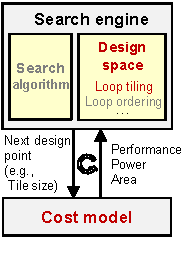
\includegraphics[width=0.3457\columnwidth]{figs/fig01_a.pdf}%
\label{fig:dse_overview_a}}
\hfil
\subfloat[]{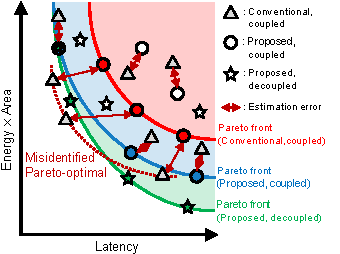
\includegraphics[width=0.6343\columnwidth]{figs/fig01_b.pdf}%
\label{fig:dse_overview_b}}
\caption{(a)~Dataflow DSE process. (b)~Impact of cost model (red vs.\ blue) and design space (blue vs.\ green).}
\label{fig:dse_overview}
\end{figure}

The latency, energy, and hardware area of a CiM accelerator are heavily dependent on the dataflow across its heterogeneous intellectual property (IP) blocks such as on-chip buffer and CiM array, in particular, loop ordering and tiling~\cite{han2023balanced_pipeline, song2025cim_dataflow}.
Therefore, design space exploration (DSE) of the dataflow is essential for optimizing CiM accelerators~\cite{he2022dse_coexploration, nettlmdse_aspdac2026, park2020roofline}.
As illustrated in Fig.~\ref{fig:dse_overview}(a), the corresponding DSE generally consists of three components: search algorithm, design space, and cost model. The search algorithm selects one of the design points in the design space, and then the latency, energy, and hardware area of the selected design point are estimated by the cost model.
The search algorithm primarily affects exploration efficiency whereas the design space and the cost model impact the optimality of the final Pareto front (given a sufficient exploration time)~\cite{schafer2020hls_dse_survey}.
When it comes to the design space for NVM-based CiM accelerators, assuming weight-stationary dataflow heavily constrains loop ordering, leaving loop tiling as a major dataflow parameter~\cite{park2025loop_tiling}.

Existing DSE approaches~\cite{maestro_micro2019, timeloop_ispass2019, zheng2023tileflow, zigzag_tc2021, wang2025atb, peng2021neurosim, eflowsim_date} remain limited in accuracy of the cost model as well as in coverage of the design space.
First, the conventional cost models tend to ignore either inter-stage pipeline stalls or memory data layout overheads, resulting in inaccurate latency/energy estimation, which may severely mislead the corresponding DSE. As illustrated in Fig.~\ref{fig:dse_overview}(b), an inaccurate cost model may misidentify non-optimal design points as Pareto-optimal (red dashed line), whereas their actual latency and energy--area product (EAP) lie in the red region. 
Second, in most of the existing approaches the design space is only confined to coupled loop tiling in which the input tile size is derived from the output tile size. As indicated by the blue region in Fig.~\ref{fig:dse_overview}(b), the limited coverage of design space through the exclusion of decoupled loop tiling may also cause the corresponding DSE to end up in non-optimal design points.

To address these limitations, the following two contributions are made in this paper:
\begin{enumerate}
\item \textbf{CiMFlowSim:} A cycle-level dataflow simulator for weight-stationary CiM accelerators. The SystemC/transaction-level modeling (TLM) simulator proposes both a dependency-aware pipeline model and a data-layout-aware memory model in order to capture both inter-stage pipeline stalls and memory data layout overheads. This simulator enables cycle-level evaluation of design points whose latency and energy diverge from analytical estimates by up to 41.1\% and 56.9\%, respectively.
\item \textbf{Decoupled loop tiling:} Decoupled loop tiling is newly considered for DSE of the dataflow for weight-stationary CiM accelerators. Also, an enumeration algorithm is provided to define the valid design space for efficient double-buffering execution.
\end{enumerate}

Experimental results evaluate the impact of the aforementioned contributions.
CiMFlowSim helps improve the estimation accuracy by up to 41.1\% in latency and 56.9\% in energy compared to the analytical cost model. When applied to loop tiling optimization, CiMFlowSim improves the hypervolume (HV)~\cite{xu2025rankdse} by up to 153.1\%, where a larger HV indicates broader coverage of the latency--EAP tradeoff space. In addition, the introduction of decoupled loop tiling into the design space further improves the HV by up to 63.7\%.

The remainder of this paper is organized as follows.
Section~\ref{sec:background} provides the background of this work and the related work.
Section~\ref{sec:decoupled_tiling} describes decoupled loop tiling for CiM accelerators, and Section~\ref{sec:cimflowsim} provides technical details of CiMFlowSim. Section~\ref{sec:results} provides experimental results on latency/energy estimation and loop tiling optimization, and Section~\ref{sec:conclusion} concludes the paper.

\section{Background and Related Work}
\label{sec:background}

Prior to discussing the technical details of this paper, this section gives an overview on the system architecture, introduces the conventional loop tiling together with the impact of memory data layout, and provides the related work.

\subsection{System Architecture}
\label{subsec:system_architecture}

Fig.~\ref{fig:system_architecture}(a) shows the block diagram of the target CiM accelerator system.
The target accelerator system typically consists of off-chip DRAM storing the activation tensors during inference, on-chip input and output SRAM buffers (IBUF and OBUF) each with double buffering for the consecutive data tiles, and a CiM array whose cells store the weights and perform multiply-and-accumulate (MAC) operations in place.
The weights remain stationary in the CiM cells, and only the input and output activations are transferred during convolution layers.
Partial sums from the CiM array are combined by an accumulation unit, and a post-processing unit applies the nonlinear activation function. This paper focuses on the dataflow, i.e., the data movement of activations, among the heterogeneous IP blocks with widely varying bandwidth and latency, e.g., the off-chip DRAM, the on-chip buffers and a CiM array. This dataflow is assumed to be controlled by input direct memory access controller (IDMAC), output direct memory access controller (ODMAC), input address-generation unit (IAGU), and output address-generation unit (OAGU). In detail, on the input side, the IDMAC and the IAGU transfer input activations from DRAM to the IBUF and from the IBUF to the CiM array, respectively. On the output side, the OAGU and the ODMAC transfer output activations from the CiM array to the OBUF and from the OBUF to DRAM, respectively. Consequently, the overall accelerator system can be seen as a 5-stage pipeline, i.e., consisting of MemRd (Stage 1), BufRd (Stage 2), CiMComp (Stage 3), BufWr (Stage 4), and MemWr (Stage 5): MemRd transfers input activations from DRAM to the IBUF and BufRd does so from the IBUF to the CiM array. Subsequently, CiMComp performs the MAC operation on the CiM array and generates a group of output activations, which is referred to as an output activation (OA) group later in this paper. Finally, BufWr writes the output activations to the OBUF, and MemWr transfers them from the OBUF to DRAM. In order to guarantee functional correctness without any violation of data dependency, both the DMACs and the AGUs should include the synchronization among the heterogeneous IP blocks~\cite{pellauer2019buffets}, which will be detailed in the later sections.

Fig.~\ref{fig:system_architecture}(b) defines the parameters for a convolutional layer.
The $M$ weight kernels of size $R \times S \times C$ are fully mapped onto the CiM array.
The input activation tensor of size $H \times W \times C$ is partitioned into input tiles of size $t_h \times t_w \times C$, and the output activation tensor of size $P \times Q \times M$ is partitioned into output tiles of size $t_p \times t_q \times M$.
Here, $h$ and $w$ denote the spatial dimensions of the input, $p$ and $q$ those of the output, and $U$ the convolution stride.
As weights are fully mapped, the weight loop is fixed and the tile sizing of input/output activations becomes the principal design parameter for DSE.

\begin{figure}[!t]
\centering
\subfloat[]{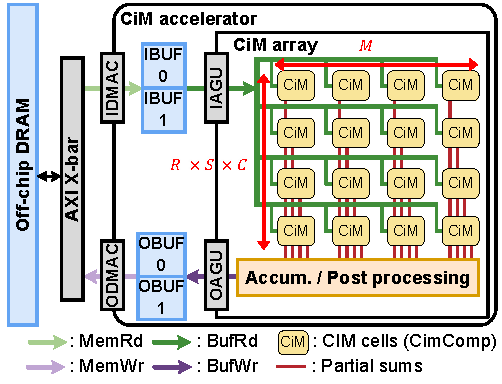
\includegraphics[width=0.6081\columnwidth]{figs/fig02_a.pdf}%
\label{fig:system_architecture_a}}
\hfil
\subfloat[]{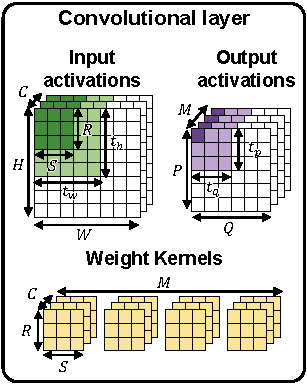
\includegraphics[width=0.3719\columnwidth]{figs/fig02_b.pdf}%
\label{fig:system_architecture_b}}
\caption{CiM accelerator architecture. (a)~Accelerator block diagram. (b)~Variable definitions for activations, weights, and tiling parameters in a convolutional layer.}
\label{fig:system_architecture}
\end{figure}

\subsection{Coupled Loop Tiling}
\label{subsec:coupled_tiling}

Although tile sizing is the principal design parameter, conventional loop tiling for DNN accelerators~\cite{maestro_micro2019, timeloop_ispass2019} defines the input tile as the region required to compute a given output tile.
As a result, the input tile size is derived from the output tile size.
Therefore, the two tile sizes are coupled and cannot be adjusted independently, with identical input and output tile sizes.
Fig.~\ref{fig:coupled_tiling} shows two coupled loop tiling examples for a layer with $H = W = 6$, $P = Q = 4$, $R = S = 3$, $C = 2$, $M = 3$, and $U = 1$.
In Fig.~\ref{fig:coupled_tiling}(a), the output tile size is $(t_p, t_q) = (2,2)$, and the corresponding input tile size is $(t_h, t_w) = (4,4)$.
Each tile iteration passes through five pipeline stages. MemRd transfers 32 pixels ($t_h \times t_w \times C$) from DRAM to the IBUF, BufRd reads 18 pixels ($R \times S \times C$) from the IBUF to the CiM array for each output pixel, CiMComp performs the MAC operation on the CiM array, BufWr writes an OA group, i.e., 3 output pixels ($M$) to the OBUF, and MemWr transfers 12 pixels ($t_p \times t_q \times M$) from the OBUF to DRAM.
Under the latency-insensitive design (LID) principle~\cite{carloni2001lid}, each IP block operates independently and communicates through asynchronous handshaking.

MemRd and MemWr operate at the tile level and each iterate $(P/t_p) \times (Q/t_q) = 4$ times.
BufRd, CiMComp, and BufWr operate at the output-pixel level and each iterate $P \times Q = 16$ times.
As shown in Fig.~\ref{fig:coupled_tiling}(a), MemRd is the latency bottleneck in this tiling.
The MemRd bottleneck can result from redundant reads of overlapping halo regions between adjacent tiles or inefficient memory access patterns owing to memory data layout.

The MemRd bottleneck can be mitigated by increasing the tile size.
In Fig.~\ref{fig:coupled_tiling}(b), the output tile size is increased to $(t_p, t_q) = (2,4)$.
The tile count decreases from 4 to 2, reducing the total number of redundant reads.
The IBUF capacity increases from 32 to 48 pixels to accommodate the larger input tile.
However, under coupled loop tiling, the OBUF capacity must also increase to 24 pixels, even though the pipeline latency is determined by MemRd, not BufWr, resulting in unnecessary buffer overhead.

\begin{figure}[!t]
\centering
\subfloat[]{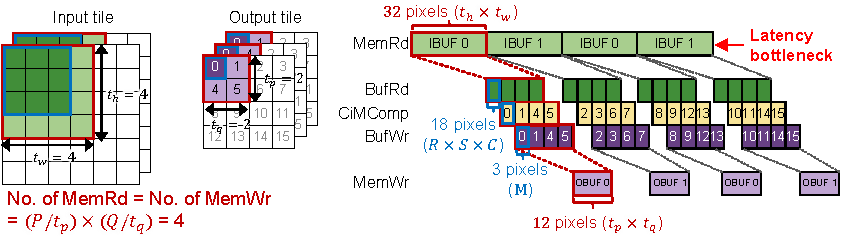
\includegraphics[width=\columnwidth]{figs/fig03_a.pdf}%
\label{fig:coupled_tiling_a}}\\
\subfloat[]{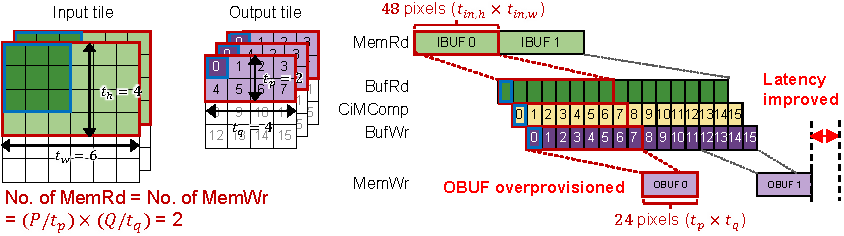
\includegraphics[width=\columnwidth]{figs/fig03_b.pdf}%
\label{fig:coupled_tiling_b}}
\caption{Coupled loop tiling examples. (a)~$(t_p, t_q) = (2,2)$. (b)~$(t_p, t_q) = (2,4)$.}
\label{fig:coupled_tiling}
\end{figure}

\subsection{Impact of Memory Data Layout}
\label{subsec:data_layout_overhead}

The memory data layout defines how each tensor element is placed on the physical memory locations, represented by a tuple of physical indices (e.g., $(\mathrm{Bank}, \mathrm{Row}, \mathrm{Column})$)~\cite{wang2024nicepim, li2022feather}. The bandwidth/latency and energy consumption of memory access are heavily dependent on the memory data layout. 

Fig.~\ref{fig:memory_layout_issues} illustrates these overheads with a $3{\times}3$ convolution on an $8{\times}8$ input ($C = 1$) under a channel-last layout, where the channel dimension is stored contiguously~\cite{wang2021dma_optimization}.
In Fig.~\ref{fig:memory_layout_issues}(a), a $4{\times}4$ input tile ($t_h = 4$, $t_w = 4$) requires 9 tiles to cover the output, reading a total of 144 elements owing to halo overlap between adjacent tiles, compared to the 64 unique input elements. Only 44.4\% of the data read by MemRd is unique.
Each input tile also maps to non-contiguous DRAM addresses, splitting the access into multiple bursts.
In Fig.~\ref{fig:memory_layout_issues}(b), the entire $8{\times}8$ input ($t_h = 8$, $t_w = 8$) is loaded at once, eliminating halo redundancy with a single contiguous burst.
However, the larger tile requires accessing 3 IBUF lines instead of 2, and the additional line access increases the BufRd latency from 1 cycle to 2 cycles.
The line utilization also drops from 56.25\% to 37.5\% as more line contents remain unused.
These two overheads, burst fragmentation and line underutilization, are tiling-dependent and are not captured by analytical cost models based on data volume alone.

\begin{figure}[!t]
\centering
\subfloat[]{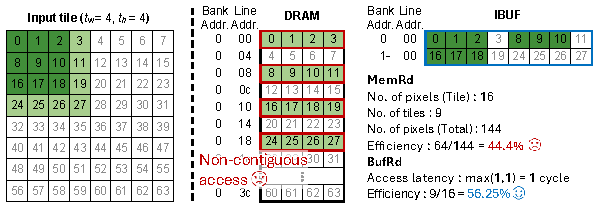
\includegraphics[width=\columnwidth]{figs/fig04_a.pdf}%
\label{fig:memory_layout_issues_a}}\\
\subfloat[]{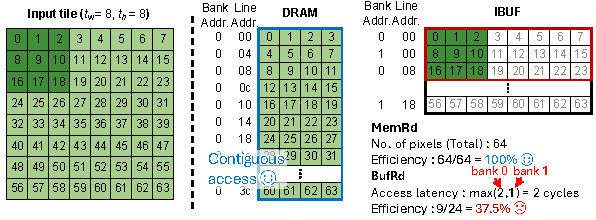
\includegraphics[width=\columnwidth]{figs/fig04_b.pdf}%
\label{fig:memory_layout_issues_b}}
\caption{Data-layout overhead for two tile sizes ($3{\times}3$ conv., $8{\times}8$ input, $C = 1$). (a)~Small tile ($t_h = 4$, $t_w = 4$). (b)~Large tile ($t_h = 8$, $t_w = 8$).}
\label{fig:memory_layout_issues}
\end{figure}

\subsection{Related Work}
\label{subsec:related_work}

Several DSE approaches have been proposed to optimize the dataflow of DNN accelerators.
The existing approaches can be mainly categorized by three technical aspects: decoupled loop tiling, dependency-aware pipeline modeling, and data-layout-aware memory modeling.

MAESTRO~\cite{maestro_micro2019}, Timeloop~\cite{timeloop_ispass2019}, and TileFlow~\cite{zheng2023tileflow} perform dataflow DSE using analytical cost models that provide rapid performance estimation from data access counts.
However, none of the aforementioned technical aspects is addressed in these approaches.
In order to improve estimation accuracy, a few existing approaches partially address dependency-aware pipeline modeling or data-layout-aware memory modeling. For example, ZigZag~\cite{zigzag_tc2021} models bandwidth-induced stalls, and FEATHER~\cite{li2022feather} accounts for on-chip data-reordering costs.
DNN+NeuroSim~\cite{peng2021neurosim} provides SPICE-calibrated circuit-level estimation for CiM accelerators, but per-component costs are still aggregated analytically without cycle-level pipeline modeling.
More importantly, the design spaces of these approaches are confined to the coupled loop tiling.

Some other approaches broaden the tiling design space by considering decoupled loop tiling.
In~\cite{wang2025atb}, the tile sizes of the input and output operands along their shared dimension are configured independently for general matrix multiplication (GEMM) on an AMD XDNA2 architecture, but the performance estimation relies on the analytical cost model based on the arithmetic intensity and the bandwidth constraints.
In~\cite{eflowsim_date}, decoupled loop tiling is newly considered for CiM accelerators, but the design space is limited to a few pre-defined loop tiling options. The absence of dependency-aware pipeline modeling and data-layout-aware memory modeling make it impossible to explore a broad design space of loop tiling for a CiM accelerator with heterogeneous IP blocks.

In summary, no existing approach concurrently addresses all the aforementioned technical aspects, to the best of the authors' knowledge. The limited cost-model accuracy and design-space coverage lead to non-optimal design points in the DSE.


\section{Decoupled Loop Tiling}
\label{sec:decoupled_tiling}

Decoupled loop tiling defines the input and output tile sizes as independent design parameters.
This expands the set of input-output tile-size combinations, enabling more flexible tradeoffs among latency, energy, and hardware area.
Algorithm~\ref{alg:decoupled_tiling} shows how to enumerate all the input-output tile-size combinations and filter out some of the less important ones.
Loop tiling is applied to $(h, w)$ for the input and $(p, q)$ for the output.
Lines~4 and~5 enumerate candidate tuples $(t_{\mathrm{in},p},\, t_{\mathrm{in},q},\, t_{\mathrm{out},p},\, t_{\mathrm{out},q})$ over the divisor sets of $P$ and $Q$.
The input tile size is expressed in output coordinates ($t_{\mathrm{in},p}$, $t_{\mathrm{in},q}$) to enable direct ratio comparison with $t_{\mathrm{out},p}$ and $t_{\mathrm{out},q}$ in the filtering conditions, and is converted to input dimensions $t_{\mathrm{in},h}$ and $t_{\mathrm{in},w}$ in Lines~14 and~15.
The enumerated candidates are then filtered by two conditions in Lines~8 and~11.
Only the remaining candidates are converted into $(t_{\mathrm{in},h},\, t_{\mathrm{in},w})$ and inserted into $\mathcal{T}$ in Lines~14--16.
Coupled loop tiling can be seen as a special case where the input and output tile sizes are dependent on each other. In more detail, the enumeration in Algorithm~\ref{alg:decoupled_tiling} is reduced into the coupled loop tiling by replacing Line~5 with $t_{\mathrm{in},p} = t_{\mathrm{out},p}$ and $t_{\mathrm{in},q} = t_{\mathrm{out},q}$.

The two filtering conditions ensure that the resulting tilings can be executed efficiently with double buffering.
First, the condition in Lines~6--9 requires the input-to-output tile count ratio in each dimension to be an integer, i.e., $1{:}M$ or $N{:}1$.
A non-integer ratio causes tile boundaries to misalign with buffer boundaries, preventing full utilization of the buffer capacity at every iteration.
Second, the condition in Lines~11--12 excludes the mixed case in which the input tile is larger than the output tile in one dimension but smaller in the other.
In such cases, data loaded into the input buffer cannot be fully reused across output tiles, and the same data must be repeatedly read from memory, increasing redundant reads.
The valid tilings enumerated by Algorithm~\ref{alg:decoupled_tiling} define the design space evaluated in this paper.

Fig.~\ref{fig:decoupled_tiling} illustrates how decoupled loop tiling combines the advantages of both cases in Fig.~\ref{fig:coupled_tiling}.
The input tile covers the same enlarged region as Fig.~\ref{fig:coupled_tiling}(b), $(t_{\mathrm{in},p}, t_{\mathrm{in},q}) = (2,4)$, reducing MemRd latency through fewer halo reads and better burst efficiency.
At the same time, the output tile remains at $(t_{\mathrm{out},p}, t_{\mathrm{out},q}) = (2,2)$ as in Fig.~\ref{fig:coupled_tiling}(a), avoiding the $2{\times}$ OBUF capacity increase.
As a result, MemRd iterates 2 times while MemWr iterates 4 times, creating mismatched tile counts across pipeline stages.
This mismatch requires the dependency-aware pipeline modeling described in Section~\ref{sec:cimflowsim}.

\begin{algorithm}[!t]
\caption{Decoupled loop tiling enumeration}
\label{alg:decoupled_tiling}
\begin{algorithmic}[1]
\STATE \textbf{Input:} $P, Q$ (output size), $R, S$ (kernel size), $U$ (stride)
\STATE \textbf{Output:} $\mathcal{T}$ (set of $(t_{\mathrm{out},p}, t_{\mathrm{out},q}, t_{\mathrm{in},h}, t_{\mathrm{in},w})$)
\STATE $\mathcal{T} \leftarrow \emptyset$
\FOR{$(t_{\mathrm{out},p}, t_{\mathrm{out},q}) \in \mathrm{Divisors}(P) \times \mathrm{Divisors}(Q)$}
\FOR{$(t_{\mathrm{in},p}, t_{\mathrm{in},q}) \in \mathrm{Divisors}(P) \times \mathrm{Divisors}(Q)$}
  \STATE $r_p \leftarrow \max(t_{\mathrm{in},p},\, t_{\mathrm{out},p}) \mathbin{/} \min(t_{\mathrm{in},p},\, t_{\mathrm{out},p})$
  \STATE $r_q \leftarrow \max(t_{\mathrm{in},q},\, t_{\mathrm{out},q}) \mathbin{/} \min(t_{\mathrm{in},q},\, t_{\mathrm{out},q})$
  \IF{$r_p \notin \mathbb{N}$ \textbf{or} $r_q \notin \mathbb{N}$} \STATE \textbf{continue} \ENDIF
  \IF{$(t_{\mathrm{in},p} - t_{\mathrm{out},p})(t_{\mathrm{in},q} - t_{\mathrm{out},q}) < 0$} \STATE \textbf{continue} \ENDIF
  \STATE $t_{\mathrm{in},h} \leftarrow R + (t_{\mathrm{in},p} - 1) \times U$
  \STATE $t_{\mathrm{in},w} \leftarrow S + (t_{\mathrm{in},q} - 1) \times U$
  \STATE $\mathcal{T} \leftarrow \mathcal{T} \cup \{(t_{\mathrm{out},p}, t_{\mathrm{out},q}, t_{\mathrm{in},h}, t_{\mathrm{in},w})\}$
\ENDFOR
\ENDFOR
\RETURN $\mathcal{T}$
\end{algorithmic}
\end{algorithm}

\begin{figure}[!t]
\centering
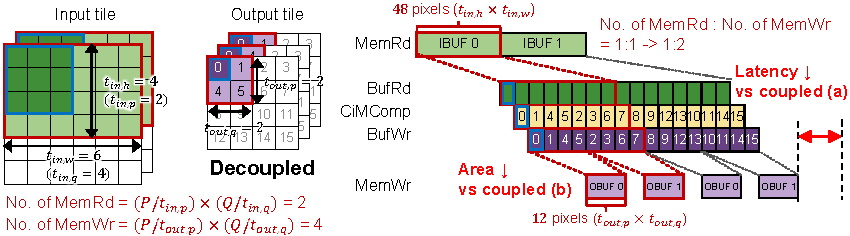
\includegraphics[width=\columnwidth]{figs/fig05.pdf}
\caption{Decoupled loop tiling example: $(t_{\mathrm{in},p}, t_{\mathrm{in},q}) = (2,4)$, $(t_{\mathrm{out},p}, t_{\mathrm{out},q}) = (2,2)$.}
\label{fig:decoupled_tiling}
\end{figure}

\section{CiMFlowSim}
\label{sec:cimflowsim}

In order to avoid any violation of data dependency among heterogeneous IP blocks (e.g., on-chip buffer and CiM array), the adjacent pipeline stages need to be synchronized to each other. Specifically, according to the producer-consumer scenario~\cite{pellauer2019buffets}, a consumer cannot read from a memory location until the producer has written to it (forward dependency). Moreover, a producer cannot write to a memory location until the consumer has read from it (backward dependency). The proposed dependency-aware pipeline modeling makes it possible to guarantee functional correctness over a broad design space of loop tiling, which includes coupled loop tiling as well as decoupled loop tiling. In addition, the bandwidth and latency of an on-chip buffer tend to be highly dependent on the data layout, which motivates us to newly propose the data-layout-aware memory modeling.

CiMFlowSim is written in SystemC/TLM~\cite{osci_systemc, doulos_tlm}, one of the natural choices for dataflow simulation~\cite{kim2020acctlmsim, wang2021dma_optimization, wang2022bus_collision, wang2022sddg, kim2021dma_estimation, eflowsim_date}. Fig.~\ref{fig:systemc_block} shows how CiMFlowSim models the target accelerator system using SystemC/TLM. Each of the IP blocks in Fig.~\ref{fig:system_architecture}(a) is implemented as an \texttt{SC\_MODULE} and connected to each other through TLM2.0 sockets, a standardized transaction interface introduced in SystemC/TLM. The dependency-aware pipeline modeling is applied to the IP components marked in green, whereas the data-layout-aware memory modeling is applied to those marked in yellow. In addition, the figure includes the completion signals used for inter-stage synchronization (e.g., \textit{BufWr\_done}, \textit{MemWr\_done}), which will be detailed later in this section. Most of the simulation models of CiMFlowSim (e.g., DMACs, on-chip buffers) were validated extensively against the register transfer level (RTL) implementations in order to prove the cycle accuracy of simulations~\cite{kim2020acctlmsim, wang2021dma_optimization, wang2022bus_collision, wang2022sddg, kim2021dma_estimation, eflowsim_date}.

\begin{figure}[!t]
\centering
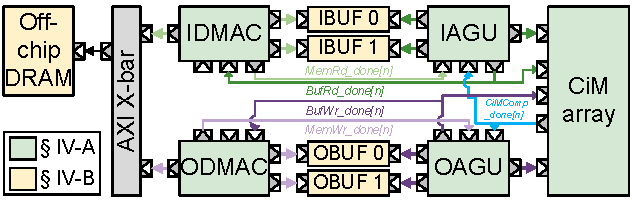
\includegraphics[width=\columnwidth]{figs/fig06.pdf}
\caption{SystemC/TLM component organization of CiMFlowSim. Bold arrows denote data paths. Thin arrows denote completion signals for inter-stage synchronization. Detailed simulation models are given in Section~\ref{subsec:pipeline_simulation} (green) and Section~\ref{subsec:memory_access_overhead} (yellow).}
\label{fig:systemc_block}
\end{figure}

\begin{table}[!t]
\centering
\caption{OAGU Internal Elements}
\label{tab:oagu_elements}
\renewcommand{\arraystretch}{1.05}
\scriptsize
\begin{tabular}{@{}llp{3.2cm}@{}}
\toprule
\textbf{Name} & \textbf{SystemC/TLM Primitive} & \textbf{Role} \\
\midrule
main\_thread & \texttt{SC\_THREAD} & Control loop over all output activation groups \\
update\_cnt & --- & Updates dependency counters on signal arrival \\
Comp\_cnt & --- & Completed CiMComp iterations (forward dep.) \\
MemWr\_cnt & --- & Completed MemWr iterations (backward dep.) \\
pl\_in/out & \texttt{tlm\_generic\_} \texttt{payload} & Activation data container \\
ev\_rd/wr & \texttt{sc\_event} & Read/write completion notification \\
nb\_fw/bw & \texttt{nb\_transport\_fw/bw} & Nonblocking transfer (CiM array$\rightarrow$OAGU$\rightarrow$OBUF) \\
t\_fw/bw\_dep & \texttt{target\_socket} & Port receiving completion signals \\
i\_in & \texttt{initiator\_socket} & Port receiving data from CiM array \\
i\_out[0/1] & \texttt{initiator\_socket} & Port sending data to OBUF (double-buffered) \\
i\_done & \texttt{initiator\_socket} & Port sending completion to adjacent stages \\
\bottomrule
\end{tabular}
\end{table}

\subsection{Dependency-Aware Pipeline Modeling}
\label{subsec:pipeline_simulation}

The synchronization between adjacent pipeline stages is performed based on the completion signals shared by the pipeline stages. A consumer checks the forward dependency by counting the assertions of the completion signal generated by a producer. Likewise, a producer checks the backward dependency by counting the assertions of the completion signal generated by a consumer. A pipeline stage continues to stall until the assertion count is above a pre-defined threshold specific to each completion signal. This makes it possible to differentiate the synchronization granularity between adjacent pipeline stages. For example, the OAGU checks the forward dependency based on \textit{CiMComp\_done} (generated by CiMComp) whereas it checks the backward dependency based on \textit{MemWr\_done} (generated by ODMAC). The synchronization with CiMComp is performed on a per-OA-group basis, whereas the one with ODMAC is on a per-output-tile basis. This dependency-aware pipeline modeling makes it possible to guarantee functional correctness over a broad design space of loop tiling including decoupled loop tiling for heterogeneous IP blocks with widely varying bandwidth and latency. 

Fig.~\ref{fig:oagu_detail} shows the internal structure of the OAGU as a representative component, and Table~\ref{tab:oagu_elements} lists its internal elements with the corresponding SystemC/TLM primitives.
The main element is main\_thread, an \texttt{SC\_THREAD} that executes the control loop.
The main\_thread receives completion signals through two \texttt{target\_socket} ports (t\_fw\_dep and t\_bw\_dep), which update the forward counter Comp\_cnt and the backward counter MemWr\_cnt via the update\_cnt callback.
Data enters through the \texttt{initiator\_socket} port i\_in from the CiM array and exits through i\_out[0] or i\_out[1] to the corresponding OBUF bank.
The transfers use \texttt{tlm\_generic\_payload} containers (pl\_in and pl\_out) and \texttt{nb\_transport\_fw/bw} nonblocking transports.
The \texttt{sc\_event} primitives ev\_rd and ev\_wr notify the main\_thread when each transaction completes, and i\_done signals completion to the adjacent components.

Fig.~\ref{fig:oagu_dependency}(a) shows the OAGU thread pseudocode, and Fig.~\ref{fig:oagu_dependency}(b) shows the resulting dependency pattern for the decoupled tiling in Fig.~\ref{fig:decoupled_tiling}, where the BufWr-to-MemWr ratio is 4:1.
The main\_thread iterates over all $P \times Q$ output activation groups.
CiMComp and BufWr each execute 16 iterations, grouped into four sets of four, where each set corresponds to one MemWr operation.
In each iteration $i$, the forward dependency check (\ding{172}) waits until the CiM array has completed the $i$-th computation ($i \geq \text{Comp\_cnt}$).
For example, BufWr[8] in Fig.~\ref{fig:oagu_dependency}(b) cannot begin until CiMComp[8] completes.
The backward dependency check (\ding{173}) waits until the ODMAC has released the target OBUF bank ($i / \text{Tile\_size} - 2 \geq \text{MemWr\_cnt}$), where the offset of 2 accounts for double buffering.
For example, BufWr[0--3] fills OBUF[0], which must be fully transferred by MemWr[0] before BufWr[8--11] can reuse the same bank.
After both conditions are met, the main\_thread reads the output activation from the CiM array, writes it to the OBUF bank selected by the double-buffering index ($i / \text{Tile\_size}) \bmod 2$, and signals completion (\ding{174}).
The same dependency logic applies to any valid tile count ratio accepted by Algorithm~\ref{alg:decoupled_tiling}.
The OBUF write latency is determined by the data-layout-aware memory model described in the next subsection.

The synchronization mechanism described above for the OAGU is not specific to this component.
Any pipeline stage can be implemented as an independent thread with its own control loop, forward and backward dependency counters driven by shared completion signals, and a tile-count ratio that determines the dependency stride.
The number and the direction of dependencies and the tile-count ratio are derived from the tiling produced by Algorithm~\ref{alg:decoupled_tiling}.
In CiMFlowSim, all five pipeline components in Fig.~\ref{fig:systemc_block} are implemented using this mechanism.
As boundary stages, MemRd has only a backward dependency, waiting for BufRd to release the IBUF, and MemWr has only a forward dependency, waiting for BufWr to fill the OBUF.

\begin{figure}[!t]
\centering
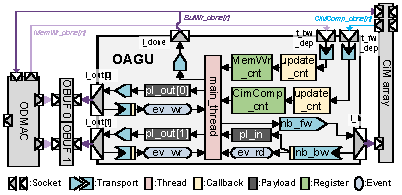
\includegraphics[width=\columnwidth]{figs/fig07.pdf}
\caption{Internal architecture of the OAGU.}
\label{fig:oagu_detail}
\end{figure}

\begin{figure}[!t]
\centering
\subfloat[]{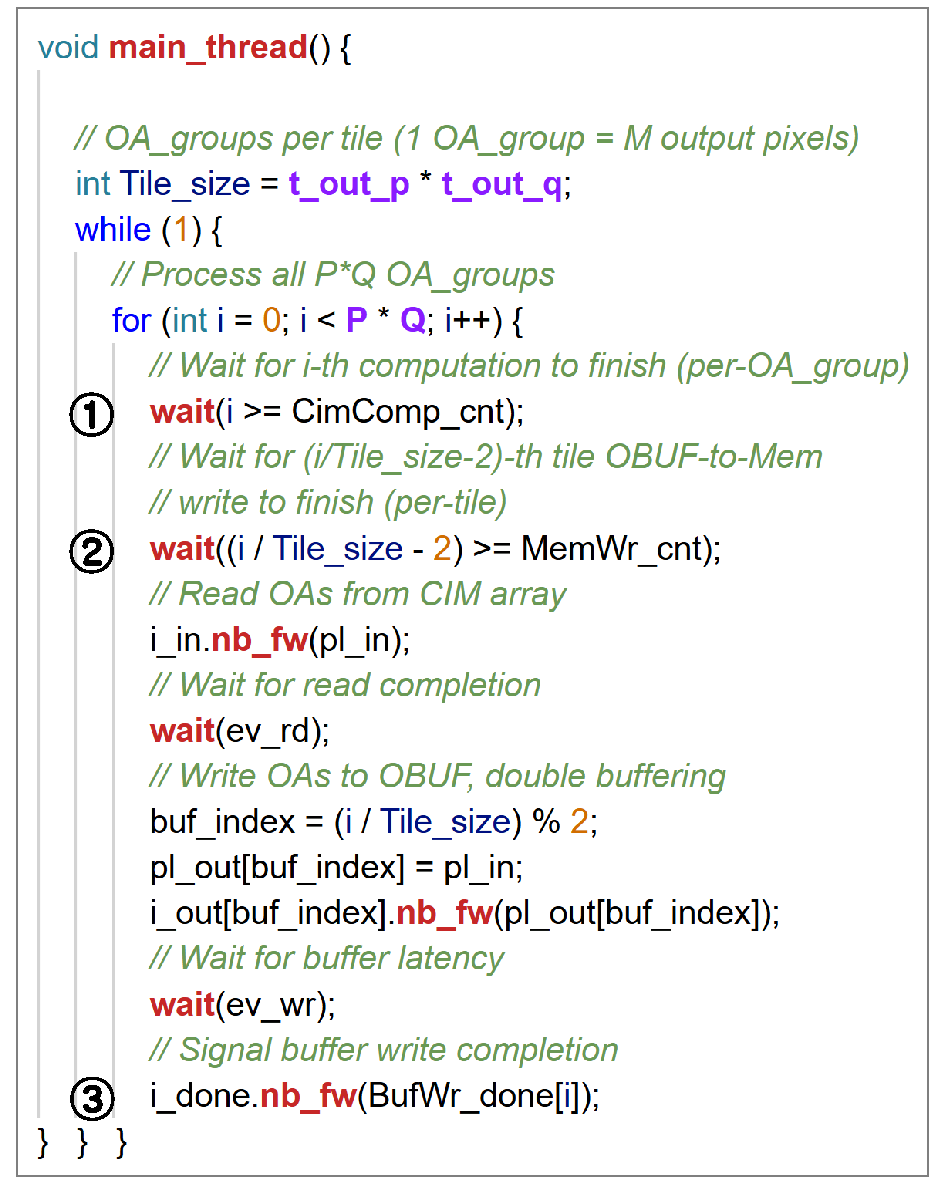
\includegraphics[width=0.75\columnwidth]{figs/fig08_a.pdf}%
\label{fig:oagu_dependency_a}}\\
\subfloat[]{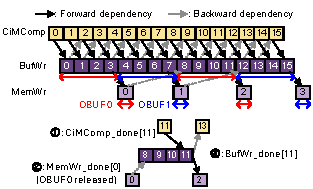
\includegraphics[width=0.9\columnwidth]{figs/fig08_b.pdf}%
\label{fig:oagu_dependency_b}}
\caption{OAGU thread behavior. (a)~Thread pseudocode. (b)~Forward and backward dependencies (BufWr:MemWr = 4:1).}
\label{fig:oagu_dependency}
\end{figure}

\subsection{Data-Layout-Aware Memory Modeling}
\label{subsec:memory_access_overhead}
The memory data layout substantially affects the bandwidth/latency and energy consumption of memory access. Most of the analytical cost models used in the existing DSE approaches~\cite{maestro_micro2019, timeloop_ispass2019, zheng2023tileflow} simply rely on the data volume in estimating the latency/bandwidth and energy consumption of memory access, i.e., without taking into account the memory data layout, which turns out to limit the estimation accuracy severely, as will be shown later in this paper. This motivates us to propose the data-layout-aware memory modeling, which contributes to improving not only the estimation accuracy but also the optimality of Pareto front.

Fig.~\ref{fig:memory_layout_flow}(a) shows the internal structure of one of the two OBUF components in Fig.~\ref{fig:systemc_block}.
Each memory component exposes two target ports and dispatches incoming transactions through per-port handlers to a central arbiter. 
The arbiter maintains two persistent data structures: \textit{tensor\_registry} stores the static placement of each tensor, and \textit{bank\_state} tracks the most recent access time of each bank.
Table~\ref{tab:memory_model_fields} lists the fields maintained by these structures.

Fig.~\ref{fig:memory_layout_flow}(b) shows the transaction sequence between the handler and the arbiter for a single tile access.
When a pipeline stage issues a tile access through t\_port[i], handler[i] receives the payload, creates a transaction containing the tensor identifier and the requested region, and submits it to the arbiter via a request event.
The arbiter checks all pending requests and selects a single request (based on a configurable policy such as FIFO or priority) since OBUF is assumed to be single-port SRAM in the target accelerator system. It is worth mentioning that the proposed memory model is generic enough to model different types of SRAM such as dual-port SRAM.
It then performs tile-to-line mapping using the tensor shape and layout from \textit{tensor\_registry}, translating the requested tile region into a set of physical line indices.
Each line is fully accessed even when only a portion of the line contains valid tile data, which accounts for line underutilization.
The arbiter waits for bank availability via \textit{bank\_state} and computes per-bank write or read latency depending on the transaction type.
In both cases, the access latency depends on the most heavily loaded bank, whereas the access energy depends on the total number of accessed lines.
The arbiter then updates \textit{tensor\_registry} and \textit{bank\_state}, annotates the transaction with the computed latency, and sends a grant event back to the handler.
When multiple ports issue requests concurrently, the arbiter serializes them by selecting one request at a time.
For example, when the OAGU in Fig.~\ref{fig:oagu_detail} writes to the OBUF through i\_out[i], the OBUF arbiter in Fig.~\ref{fig:memory_layout_flow} computes the access latency and returns it via the ev\_wr event, which the OAGU thread uses to advance the simulation time.

The memory model described above for the OBUF is instantiated for every memory component in Fig.~\ref{fig:systemc_block}, including both IBUF banks and the off-chip DRAM.
All instances share the same arbiter logic, namely tensor registration, tile-to-line mapping, per-bank line counting, and max-loaded-bank latency computation.
The instances differ only in configuration parameters such as clock frequency, base access latency, line width, and bank count.
The registered tensor shapes also differ. On-chip buffers register tile-sized tensors determined by the tiling, whereas DRAM registers full activation maps.
The access logic resides entirely in the arbiter, and reconfiguring a memory component requires only a different set of parameters.

\begin{figure}[!t]
\centering
\subfloat[]{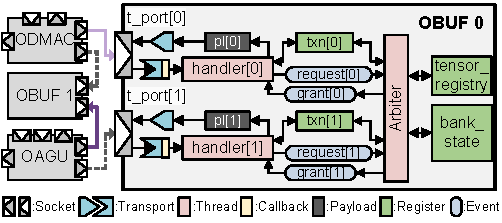
\includegraphics[width=\columnwidth]{figs/fig09_a.pdf}%
\label{fig:memory_layout_flow_a}}\\
\subfloat[]{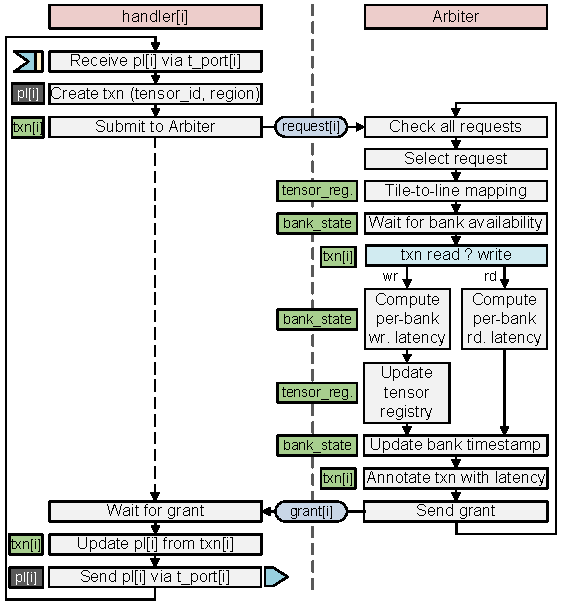
\includegraphics[width=\columnwidth]{figs/fig09_b.pdf}%
\label{fig:memory_layout_flow_b}}
\caption{Data-layout-aware memory model for OBUF. (a)~Internal structure. (b)~Transaction sequence.}
\label{fig:memory_layout_flow}
\end{figure}

\begin{table}[!t]
\centering
\caption{Access-Model State Fields}
\label{tab:memory_model_fields}
\renewcommand{\arraystretch}{1.15}
\footnotesize
\begin{tabular}{@{}lp{5.0cm}@{}}
\toprule
\textbf{Field} & \textbf{Description} \\
\midrule
\multicolumn{2}{@{}l}{\textit{tensor\_registry} (per tensor)} \\
\quad id & Tensor identifier \\
\quad shape & Tensor dimensions \\
\quad bitwidth & Bits per element \\
\quad layout & Data layout \\
\quad bank\_range & Allocated bank indices \\
\quad line\_base & Starting physical line index \\
\quad elements\_per\_line & Tensor elements packed per physical line \\
\midrule
\multicolumn{2}{@{}l}{\textit{bank\_state} (per bank)} \\
\quad last\_access\_time & Most recent access completion time \\
\bottomrule
\end{tabular}
\end{table}

\section{Experimental Results}
\label{sec:results}

This section evaluates the estimation accuracy of CiMFlowSim and the impact of decoupled loop tiling on DSE results.
Experiments are conducted on two NVM-based CiM accelerators whose architectural parameters are summarized in Table~\ref{tab:hardware_config}.
Both accelerators use LPDDR4-3200 off-chip memory with a bandwidth of 6.4\,GB/s.
Four convolutional neural network (CNN) benchmarks are evaluated: LeNet-5~\cite{lecun1998lenet}, VGG-11~\cite{simonyan2015vgg}, MobileNetV1~\cite{howard2017mobilenet}, and ResNet-18~\cite{he2016resnet}.
The MobileNetV1 evaluation excludes depthwise layers, as depthwise convolutions are inefficient under the weight-stationary dataflow assumed in this work.
The analytical cost model used as the baseline is based on MAESTRO~\cite{maestro_micro2019} and is adjusted to match the target hardware in Table~\ref{tab:hardware_config}.

For a network with $N$ convolutional layers, the total latency and energy are $L_{\mathrm{net}} = \sum_{\ell=1}^{N} L_{\ell}$ and $E_{\mathrm{net}} = \sum_{\ell=1}^{N} E_{\ell}$, whereas the required on-chip buffer area is $A_{\mathrm{net}} = \max_{\ell} A_{\ell}$.
The two DSE objectives are latency and the energy--area product, $\mathrm{EAP}_{\mathrm{net}} = E_{\mathrm{net}} \times A_{\mathrm{net}}$, where $E_{\mathrm{net}}$ sums the energy consumed in off-chip DRAM, the on-chip buffers, and the CiM array.
In terms of area, tiling decisions affect only the buffer requirements.
Therefore, $A_{\mathrm{net}}$ denotes only the required on-chip buffer area, as all other hardware blocks remain fixed.
Since the number of all per-layer tiling combinations grows exponentially with the number of layers, the network-level Pareto front is approximated by randomly sampling 100 million tiling combinations, where each sample selects one valid tiling per layer and computes the network-level latency and EAP.
The sample count was determined empirically, as further increases did not change the resulting HV rankings.

Pareto front quality is measured by HV~\cite{xu2025rankdse}.
Each Pareto-optimal point dominates the rectangular region between itself and a reference point, and HV is the union area of all such regions.
A larger HV indicates a Pareto front that covers a wider range of the objective space with better tradeoffs.
In this work, HV is computed in the two-dimensional space of (latency, EAP).
The reference point for each hardware-network pair is set to 5\% above the worst latency and EAP among the Pareto-optimal points across the compared methods.
HV is normalized by the rectangular area formed by the reference point and the point $(L_{\mathrm{best}}, \mathrm{EAP}_{\mathrm{best}})$, where $L_{\mathrm{best}}$ and $\mathrm{EAP}_{\mathrm{best}}$ are the best observed latency and EAP independently across all Pareto-optimal points.

\begin{table}[!t]
\caption{Evaluated CiM Accelerator Hardware Parameters}
\label{tab:hardware_config}
\centering
\small
\begin{tabular}{lcc}
\toprule
\textbf{Parameter} & \textbf{MRAM}~\cite{chiu2023isscc_mram} & \textbf{eFlash}~\cite{choi2023cicc_eflash} \\
\midrule
Process Node & 22\,nm & 65\,nm \\
Macro Array Size (I$\times$O) & 576$\times$72 & 32$\times$64 \\
Compute Latency & 20\,ns & 50\,ns \\
Energy Efficiency & 46\,TOPS/W & 333\,TOPS/W \\
\bottomrule
\end{tabular}
\end{table}

\subsection{Estimation Error Analysis}
\label{subsec:prediction_error}

This subsection analyzes the estimation errors of the analytical cost model and their impact on DSE results.

Fig.~\ref{fig:tile_error_heatmap} shows the latency estimation error of the analytical cost model relative to CiMFlowSim over the two-dimensional space of input and output tile sizes for (MRAM, VGG-11, Layer~0).
The error ranges from near zero to 37.7\% across tilings, indicating that it is tiling-dependent rather than a uniform bias.
Low-error and high-error regions are scattered across the tile-size space, and no monotonic trend is observed along either axis.
This tiling-dependent error is unlikely to be corrected by applying a single calibration factor to the analytical cost model and may cause the DSE to end up with non-optimal design points.

\begin{figure}[!t]
\centering
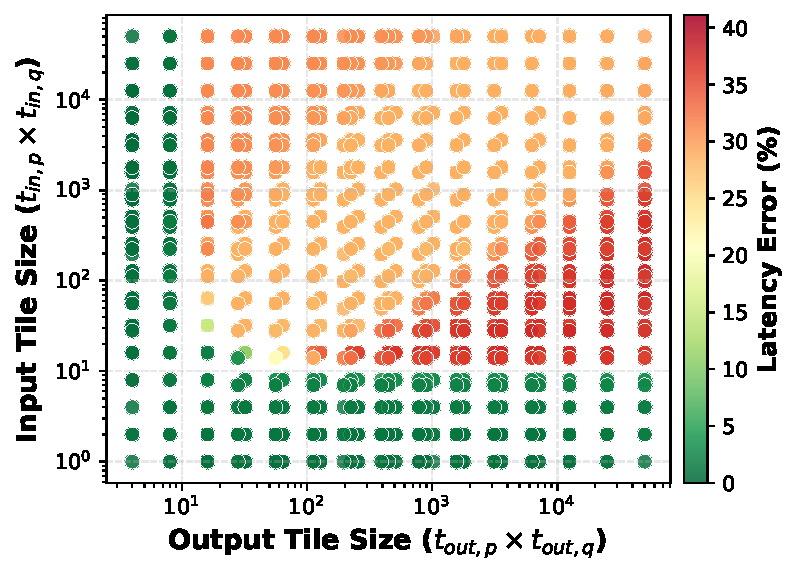
\includegraphics[width=0.75\columnwidth]{figs/fig10.pdf}
\caption{Latency estimation error over the two-dimensional tile-size space (MRAM, VGG-11, Layer~0).}
\label{fig:tile_error_heatmap}
\end{figure}

Fig.~\ref{fig:prediction_error_bar} shows the latency and energy estimation errors of the analytical cost model relative to CiMFlowSim across all hardware-network pairs.
The deviations are observed in every case, with maximum latency errors ranging from 10.8\% to 41.1\% and maximum energy errors from 18.3\% to 56.9\%.
The large gap between mean and maximum values confirms that the tiling-dependent error observed in Fig.~\ref{fig:tile_error_heatmap} persists across all evaluated configurations. 
\begin{figure}[!t]
\centering
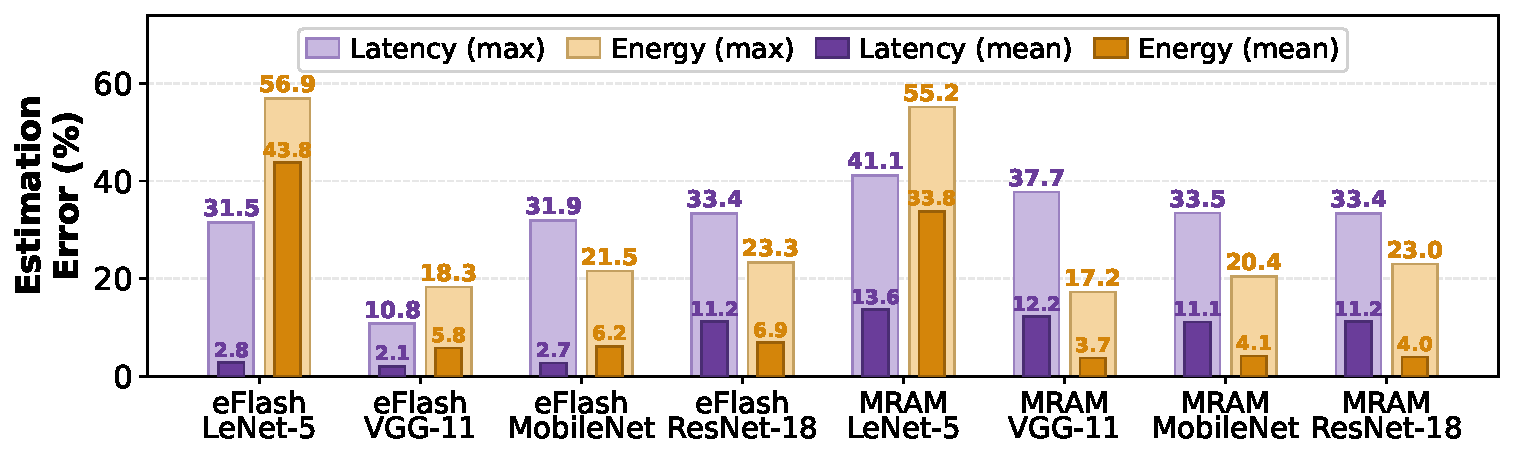
\includegraphics[width=\columnwidth]{figs/fig11.pdf}
\caption{Analytical latency and energy estimation errors across all hardware-network pairs. Thin bars denote mean relative error. Wide bars denote maximum relative error.}
\label{fig:prediction_error_bar}
\end{figure}

To assess whether these estimation errors affect network-level DSE results, the Pareto fronts obtained by the analytical baseline and CiMFlowSim are compared.
Fig.~\ref{fig:analytical_vs_simulation} shows all coupled loop tilings for (MRAM, LeNet-5) evaluated by both methods at the network level, where blue circles represent CiMFlowSim and red circles represent the analytical baseline.
In Fig.~\ref{fig:analytical_vs_simulation}(a), the analytical Pareto-optimal points (red stars) appear closer to the origin than the CiMFlowSim Pareto-optimal points (blue stars), suggesting lower latency and lower EAP.
Since the analytical cost model suffers from the estimation errors shown above, this apparent advantage may not be reliable.
In Fig.~\ref{fig:analytical_vs_simulation}(b), the Pareto region is shown in detail, and the analytical Pareto-optimal points are re-evaluated with CiMFlowSim (red triangles).
The re-evaluated points shift toward higher latency and higher EAP, confirming that the analytical cost model underestimates the latency and the EAP of these design points.
As a result of this shift, rank reversals occur, and design points with lower latency and EAP may be missed.
HV improves from 0.435 to 0.595 (+36.8\%) when the Pareto front is re-evaluated with CiMFlowSim.

\begin{figure}[!t]
\centering
\subfloat[]{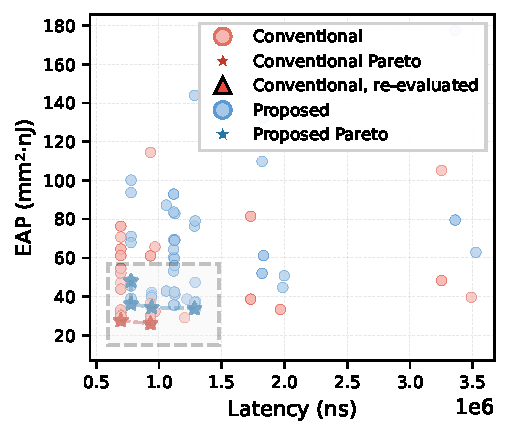
\includegraphics[width=0.49\columnwidth]{figs/fig12_a.pdf}%
\label{fig:analytical_vs_simulation_a}}
\hfil
\subfloat[]{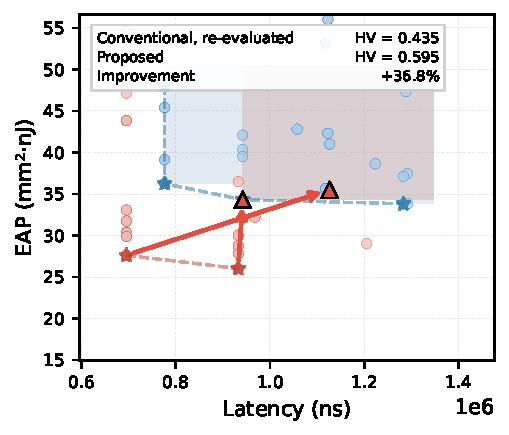
\includegraphics[width=0.49\columnwidth]{figs/fig12_b.pdf}%
\label{fig:analytical_vs_simulation_b}}
\caption{Coupled loop tilings evaluated analytically and with CiMFlowSim (MRAM, LeNet-5). (a)~All network-level points. (b)~Pareto region (detail). Arrows show re-evaluated analytical Pareto points.}
\label{fig:analytical_vs_simulation}
\end{figure}

Fig.~\ref{fig:hv_bar} reports normalized HV across all evaluated hardware-network pairs.
CiMFlowSim improves HV by up to 153.1\% (eFlash, ResNet-18).
The largest improvement occurs for ResNet-18, where the greater number of layers increases the likelihood of per-layer estimation errors affecting the network-level Pareto front.
By contrast, the HV difference is near zero for (eFlash, VGG-11) and (eFlash, MobileNetV1).
Although the analytical cost model still exhibits errors for these cases (Fig.~\ref{fig:prediction_error_bar}), small tiles do not increase the pipeline latency when the compute stage is dominant.
Therefore, the selected tilings have low estimation error, reducing the chance of rank reversals.

\begin{figure}[!t]
\centering
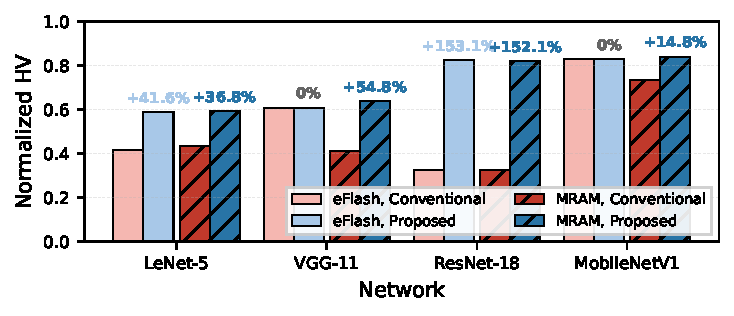
\includegraphics[width=\columnwidth]{figs/fig13.pdf}
\caption{Normalized hypervolume of coupled loop tilings across all evaluated hardware-network pairs: Analytical vs.\ CiMFlowSim.}
\label{fig:hv_bar}
\end{figure}

\subsection{Loop Tiling Optimization}
\label{subsec:decoupled_evaluation}

The previous subsection has shown the need for an accurate cost model.
This subsection evaluates the effect of expanding the tiling design space through decoupled loop tiling.

Fig.~\ref{fig:decoupled_analysis}(a) and~(b) show all coupled (blue) and decoupled (green) loop tilings for Layer~0 and Layer~1 of (MRAM, LeNet-5), respectively, in the latency--EAP space.
At the per-layer level, the decoupled loop tilings extend the design space beyond the coupled loop tilings, though the effect on the per-layer Pareto front appears limited.
At the network level, latency and energy are accumulated across layers while buffer area is determined by the single largest layer ($A_{\mathrm{net}} = \max_{\ell} A_{\ell}$).
Therefore, the network-level Pareto front depends on the combination of per-layer tiling selections, and a wider range of tradeoffs can be achieved than any single layer suggests.
Fig.~\ref{fig:decoupled_analysis}(c) compares the resulting network-level Pareto fronts.
The inclusion of decoupled loop tiling increases HV from 0.595 to 0.927 (+55.8\%) by introducing design points with lower EAP.
Under decoupled loop tiling, the input and output tile sizes are set independently, allowing the most area-demanding layer to reduce its buffer requirement without increasing latency.
As a result, the Pareto front is extended into a region not covered by coupled loop tiling.

Two design points with nearly identical latency are selected from the coupled and decoupled Pareto fronts in Fig.~\ref{fig:decoupled_analysis}(c), marked with circles.
These two points differ only in the Layer~1 tiling.
Fig.~\ref{fig:cycle_traces} compares the cycle traces of Layer~1 for these two points.
In the decoupled case, a smaller input tile is used, which requires fewer IBUF lines and reduces the buffer area by 32\%.
However, the decoupled tiling incurs more MemRd iterations owing to redundant reads of overlapping halo regions, increasing the energy by 25\%.
The additional MemRd iterations overlap with the bottleneck stage, and the overall latency is not increased.
As a result, the per-layer energy increase has a smaller impact on the network-level EAP than the buffer area reduction.

\begin{figure}[!t]
\centering
\subfloat[]{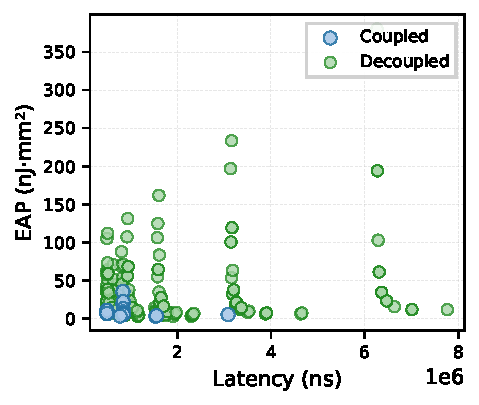
\includegraphics[width=0.49\columnwidth]{figs/fig14_a.pdf}%
\label{fig:decoupled_analysis_a}}
\hfil
\subfloat[]{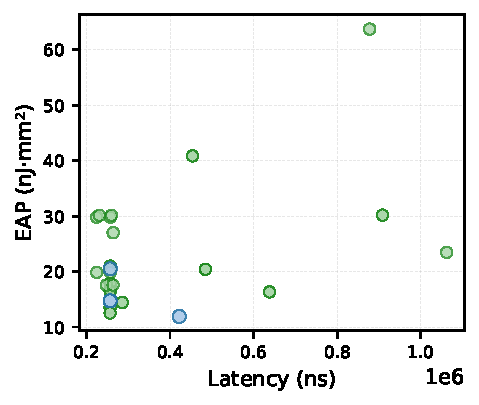
\includegraphics[width=0.49\columnwidth]{figs/fig14_b.pdf}%
\label{fig:decoupled_analysis_b}}\\
\subfloat[]{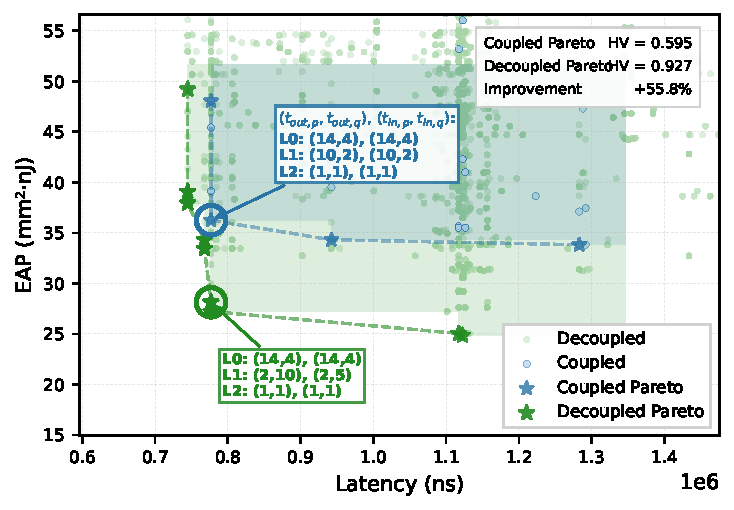
\includegraphics[width=0.85\columnwidth]{figs/fig14_c.pdf}%
\label{fig:decoupled_analysis_c}}
\caption{Effect of decoupled loop tiling (MRAM, LeNet-5) in the latency--EAP space. (a)~Layer~0. (b)~Layer~1. (c)~Network-level.}
\label{fig:decoupled_analysis}
\end{figure}

\begin{figure}[!t]
\centering
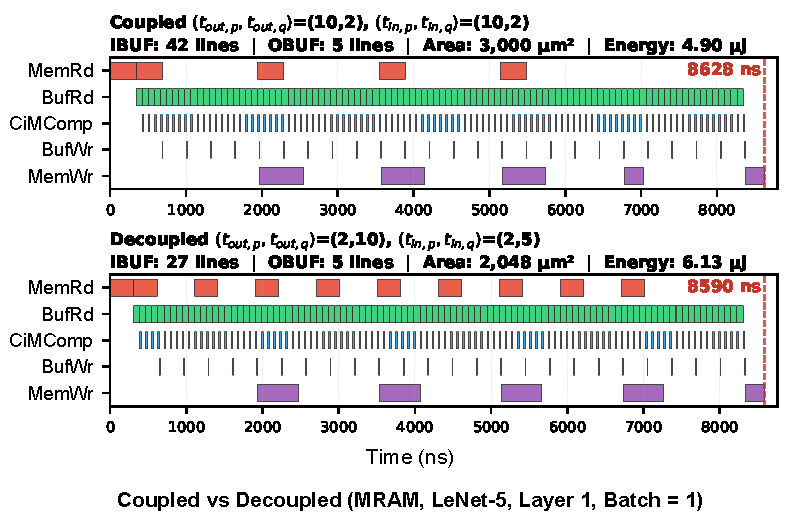
\includegraphics[width=\columnwidth]{figs/fig15.pdf}
\caption{Cycle traces of coupled and decoupled design points at nearly identical latency (MRAM, LeNet-5, Layer~1).}
\label{fig:cycle_traces}
\end{figure}

Whether the HV gain holds across all hardware-network pairs is examined next. Fig.~\ref{fig:hv_comparison} reports the results for all evaluated pairs.
The maximum HV gain of 63.7\% is observed for (eFlash, LeNet-5).
By contrast, the HV gain for (eFlash, VGG-11) is near zero.
When the compute stage dominates the pipeline latency, the memory stages have a reduced impact on the overall latency, leaving limited room for tile sizing to improve the Pareto front.

\begin{figure}[!t]
\centering
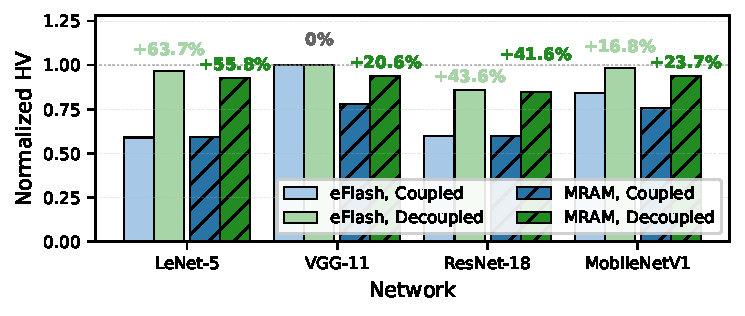
\includegraphics[width=\columnwidth]{figs/fig16.pdf}
\caption{Normalized hypervolume across all evaluated hardware-network pairs. Coupled vs.\ decoupled loop tiling. Percentages denote HV gain from decoupled loop tiling.}
\label{fig:hv_comparison}
\end{figure}

\section{Conclusion}
\label{sec:conclusion}

In this paper, CiMFlowSim, a cycle-level dataflow simulator for weight-stationary CiM accelerators, has been presented.
The proposed simulator employs a dependency-aware pipeline model to capture inter-stage pipeline stalls and a data-layout-aware memory model to account for memory data layout overheads.
In addition, decoupled loop tiling is incorporated into the weight-stationary CiM pipeline so that the input and output tile sizes can be configured independently, thereby expanding the design space beyond conventional coupled tiling.
Experimental results show that the estimation error of the analytical cost model amounts to 41.1\% in latency and 56.9\% in energy.
These tiling-dependent errors cannot be corrected by a single calibration factor and may cause the DSE to end up with non-optimal design points.
When applied to loop tiling optimization, CiMFlowSim improves the hypervolume by up to 153.1\%.
In addition, incorporating decoupled loop tiling into the design space leads to the HV gain of up to 63.7\%.
These results demonstrate that both cost-model accuracy and design-space coverage are of primary importance in the DSE of CiM accelerators.


\bibliographystyle{IEEEtran}
\bibliography{mybib}

\begin{IEEEbiography}[{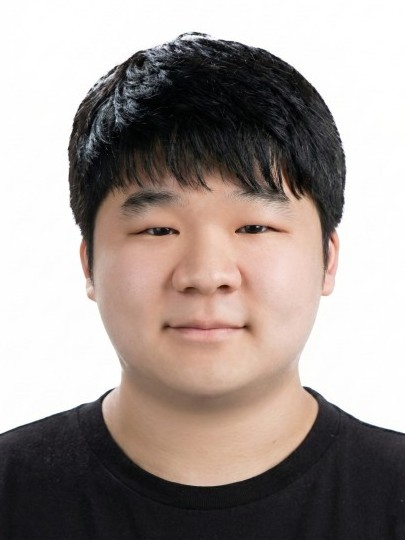
\includegraphics[width=1in,height=1.25in,clip,keepaspectratio]{figs/bio_junsu_heo.jpg}}]{Junsu Heo} received the B.S. and M.S. degrees in electrical and electronics engineering from Konkuk University, Seoul, South Korea, where he is currently pursuing the Ph.D. degree.

His research interests include SoC architecture design, virtual-prototype-based system simulation, and algorithm-hardware co-optimization.
\end{IEEEbiography}

\begin{IEEEbiography}[{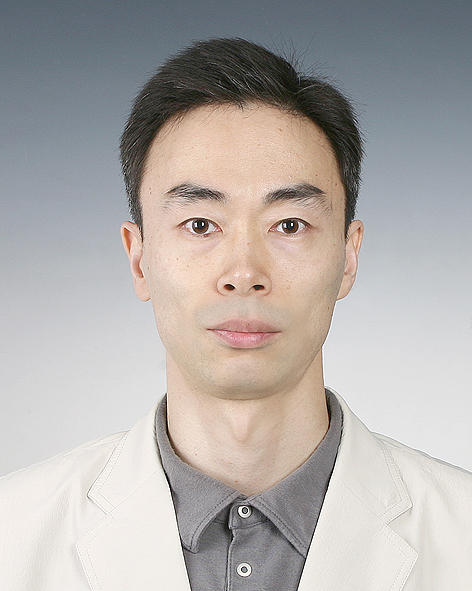
\includegraphics[width=1in,height=1.25in,clip,keepaspectratio]{figs/bio_sungkyung_park.png}}]{Sungkyung Park} (Senior Member, IEEE) received the B.S., M.S., and Ph.D. degrees all from Seoul National University, South Korea.

From 2002 to 2004, he was with Samsung Electronics, Suwon, Korea, as a Senior Engineer, where he worked on the development of system-level simulators for cellular standards. From 2004 to 2006, he was with Electronics and Telecommunications Research Institute (ETRI), Daejeon, Korea, as a Senior Member of Research Staff, where he worked on the fiber-optic front-end IC design. From 2006 to 2009, he was with Ericsson Inc., as a Senior Staff Hardware Designer, where he worked on the design and modeling of multi-standard RF transceivers and clocking circuits. In 2009, he joined the Faculty of the Department of Electrical and Electronics Engineering, Pusan National University, Busan, South Korea, where he is currently a Professor.

His research interests include SoC modeling and design, hardware accelerator and processor design, and virtual platform development for AI and wireless communication.
\end{IEEEbiography}

\begin{IEEEbiography}[{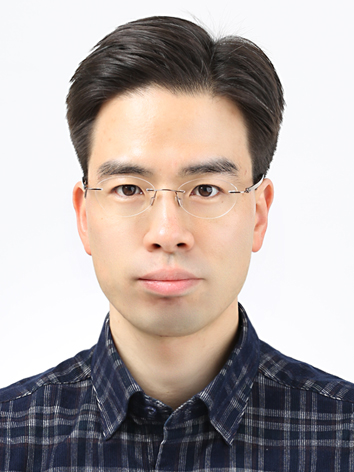
\includegraphics[width=1in,height=1.25in,clip,keepaspectratio]{figs/bio_chester_park.jpg}}]{Chester Sungchung Park} (Senior Member, IEEE) received the B.S., M.S., and Ph.D. degrees in electronics engineering all from Korea Advanced Institute of Science and Technology (KAIST), Daejeon, South Korea.

From 2006 to 2007, he was with Samsung Electronics, Giheung, South Korea, as a Senior Engineer, where he worked on flash memory controller including error correction codes. From 2007 to 2013, he was with Ericsson Research, CAL, USA, as a Senior Engineer, where he worked on wireless communication algorithms, circuit modeling, and the relevant 3GPP standardizations. Since 2013, he has been with the Department of Electrical and Electronics Engineering, Konkuk University, Seoul, South Korea, where he is currently working on algorithm-architecture co-optimizations using virtual prototype based system simulations.
\end{IEEEbiography}

\end{document}
